\section{Background Information}


\subsection{Kinect}

\subsubsection{Overview}
The Kinect was developed and launched in 2010 by Microsoft. At the time of its release, it revolutionised depth acquisition technology as it was the first depth sensing device that was available to the consumer market. This low-cost, freely available technology made depth sensing accessible and caused an explosion in the use of of depth data for various applications. \cite{kinectComp2011}

\subsubsection{Versions}

\paragraph{Kinect for Xbox 360}
The first generation Kinect was launched in 2010. It was released for the Xbox 360 gaming console. It is officially called the Kinect for Xbox 360. \cite{kinectComp2011} A picture can be seen in Figure \ref{fig:kinect360}. However, it is referred to by various names in different literature. Below are different names used to refer to the Kinect for Xbox 360:

\begin{figure}[ht]
	\centering
	{%
		\setlength{\fboxsep}{0pt}%
		\setlength{\fboxrule}{0.5pt}%
		\fbox{
			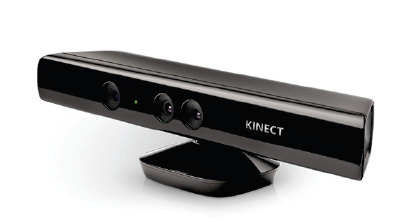
\includegraphics[width=0.7\textwidth]{Kinect360.png}
	}}
	\caption{Kinect for Xbox 360 \cite{kinectComp2011}}
	\label{fig:kinect360}
\end{figure}

\begin{itemize}
	\item First Generation Kinect 
	\item Kinect Version 1 (v1)
	\item Xbox Kinect 360 
\end{itemize} 

\paragraph{Kinect for Xbox One}
The second generation Kinect was launched in 2013. It was released with the Xbox One gaming console and is, thus, officially called the Kinect for Xbox One. \cite{kinectComp2011} A picture can be seen in Figure \ref{fig:kinectOne}. It is also referred to by different names, which are listed below for completeness:

\begin{figure}[ht]
	\centering
	{%
		\setlength{\fboxsep}{0pt}%
		\setlength{\fboxrule}{0.5pt}%
		\fbox{
			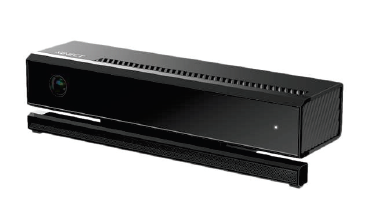
\includegraphics[width=0.7\textwidth]{KinectOne.png}
	}}
	\caption{Kinect for Xbox One \cite{kinectComp2011}}
	\label{fig:kinectOne}
\end{figure}

\begin{itemize}
	\item Second Generation Kinect 
	\item Kinect Version 2 (v2)
	\item Xbox Kinect One 
\end{itemize} 

\paragraph{Kinect for Windows}
For each generation of Kinect for Xbox released, a Kinect for Windows was released. The version numbers correlate (I.e. The Kinect for Windows also has a v1 and v2). Kinect for Windows was created to be used by a computer whereas the Kinect for Xbox to be used by the console. They are, however, functionally identical and thus, a Kinect for Xbox can be "converted" to a  Kinect for Windows by using a USB adapter. The only difference with this is that the Kinect for Windows supports "Near Mode" whereas a Kinect for Xbox used with an adapter does not. ("Near Mode" will be explained further in Section \hl{(Near Mode explanation)})

\paragraph{Kinect Used}
In this project, the Kinect for Xbox 360 with a USB adapter was used for development. Further reasons for this component choice is given in Section \hl{(Component Selection)}

\subsubsection{Components and Specifications} \label{kinectCompSpecs}
The Kinect for Windows (Kinect for Xbox 360 with a USB adapter) consists of a stand and a housing for the sensing components. Between the housing and a stand is a motor that is able to adjust the vertical tilt of the housing. The Kinect is able to achieve a maximum viewing angle of $43^{\circ}$ vertical by $57^{\circ}$ horizontal. It also has a vertical tilt range of $\pm27^{\circ}$. \cite{msdnKinectSpecs2017}

The housing contains the following main components:

\begin{itemize}
	\item An RGB Camera or Colour Sensor
	\item An IR Emitter
	\item An IR Depth Sensor
	\item A Microphone Array
	\item A 3-axis Accelerometer
\end{itemize}

The configuration of the stand, housing and internal components can be seen in Figure \ref{fig:kinectComponents}. A more detailed explanation of each of the components necessary for this project is included below:

\begin{figure}[ht]
	\centering
	{%
		\setlength{\fboxsep}{0pt}%
		\setlength{\fboxrule}{0.5pt}%
		\fbox{
			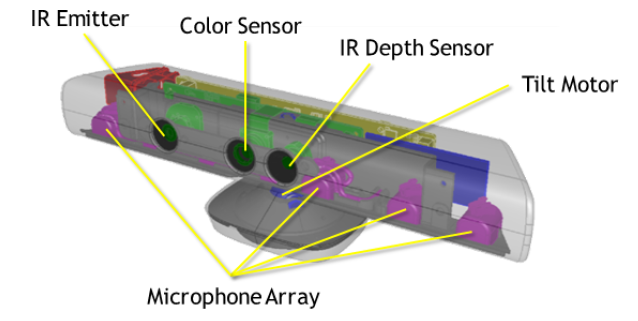
\includegraphics[width=0.7\textwidth]{Kinect360Components.png}
	}}
	\caption{Internal component layout of the Kinect for Xbox 360 \cite{msdnKinectSpecs2017}}
	\label{fig:kinectComponents}
\end{figure}

\paragraph{Colour Sensor}
The RGB camera has a maximum resolution of 1280 x 960 pixels. Each pixel is able to store red, green and blue data, allowing the camera to capture a colour image. \cite{msdnKinectSpecs2017}

\paragraph{Depth Sensor}
The depth sensor is made up of an infrared (IR) Emitter and an IR depth sensor. The emitter projects infrared light beams across the entire field of view of the Kinect. These beams hit various surfaces across the field of view and are reflected back at the Kinect. The IR depth sensor detects these reflected beams and converts them into depth data indicating the distance between the Kinect and a particular object. The collection and processing of all the reflected beams enables the Kinect to produce depth images with a maximum resolution of 640 x 480 depth image pixels. \cite{msdnKinectSpecs2017} An extension on the depth sensor is provided in the section below if more information on the intricacies of the depth sensor is required:

\subparagraph{Extension on Depth Sensor}
The depth sensor relies on a principle known as structured light. The IR emitter projects a light pattern at a wavelength of 830 nm that form an image of pseudo-random located dots. The IR depth sensor, which is an IR video-camera, also runs on a wavelength of 830 nm and can detect the light pattern. The Kinect also possesses a reference pattern that displays the light pattern at a fixed distance. This pattern is used for calibration and is used to determine depth by comparing the reflected light pattern detected with the reference pattern. \cite{kinectComp2011} This is illustrated in Figure \ref{fig:depthRefPattern}.

\begin{figure}[ht]
	\centering
	{%
		\setlength{\fboxsep}{0pt}%
		\setlength{\fboxrule}{0.5pt}%
		\fbox{
			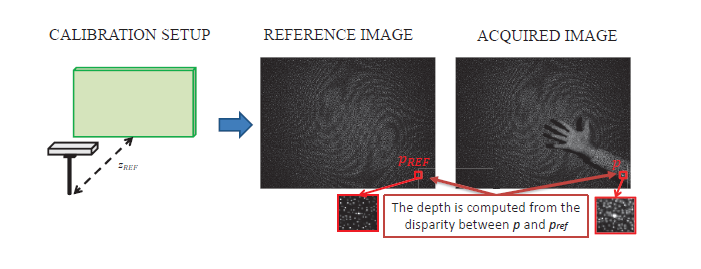
\includegraphics[width=0.7\textwidth]{depthSensorReferencePattern.png}
	}}
	\caption{An illustration of the process used by the depth sensor to determine depth by comparing the reference image to the detected one. \cite{kinectComp2011}}
	\label{fig:depthRefPattern}
\end{figure}

\subsubsection{Coordinate Spaces}
The Kinect is able to stream 3 types of data - colour, depth and skeleton data. This streamed data is available in the form of data frames that occur one at a time. The Kinect API also provides functionality that converts data between the different spaces. \cite{msdnCoSpaces2017} The sections below will elaborate on each of the spaces and will conclude with a synopsis of the conversion functionality available:

\paragraph{Colour Space}
The colour sensor is able to produce frames at a rate of 30 frames per second (fps). \cite{msdnKinectSpecs2017} Each frame captured consists of the colour image of everything inside the field of view of the colour sensor. The frame is made of pixels. As mentioned in \ref{kinectCompSpecs}, these pixels hold red, blue and green data. The number of pixels in the image depends on the resolution selected and each pixel is uniquely identified by an (x, y) coordinate. These (x, y) coordinates form the colour space. \cite{msdnCoSpaces2017}

\paragraph{Depth Space}
Similarly to the the colour sensor, the depth sensor is also able to produce frames at a rate of 30 fps. \cite{msdnKinectSpecs2017} Each frame captured also retains the information of everything in the field of view of the depth sensor and is in the form of pixels, whose size is determined by the resolution selected.  However, the difference with the depth sensor is that the data captured is a grayscale image and each pixel at a particular (x, y) coordinate, contains the Cartesian distance in millimetres from the camera plane to the nearest object, instead of red, blue and green data. The mapping of the distances to the depth space can be seen in Figure Much like the colour space, the collection of (x, y) coordinates form the depth space (I.e. The location of the depth pixels in the depth frame). The (x, y) coordinates, therefore, do not correspond to physical or Cartesian coordinates in the real world. \cite{msdnCoSpaces2017}

\begin{figure}[ht]
	\centering
	{%
		\setlength{\fboxsep}{0pt}%
		\setlength{\fboxrule}{0.5pt}%
		\fbox{
			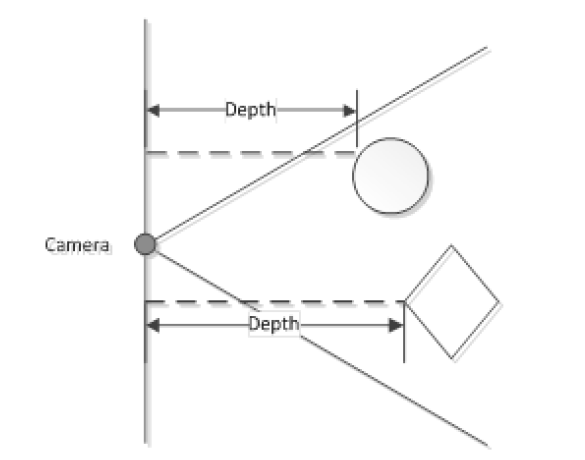
\includegraphics[width=0.7\textwidth]{distanceToDepthSpace.png}
	}}
	\caption{An illustration of the distances that stored in each depth pixel, at a particular (x, y) coordinate. \cite{msdnCoSpaces2017}}
	\label{fig:distanceToDepthSpace}
\end{figure}

\subparagraph{Range}

\subparagraph{Depth Data Storage}

\paragraph{Skeleton Space}

Conversion to 3D space \cite{nonContact2017}\\

\subparagraph{3D Points - No calibration}

\paragraph{Conversion}

\subsubsection{Internal Process}
Middleware \cite{nonContact2017}\\
Joint Filtering\\

\subsubsection{Skeleton Tracking}
Skeleton tracking\\
Known errors\\
Guidelines for measurements\\

\subsubsection{Noise}




\subsection{Microsoft SDK}

\subsubsection{Digital Information}

\subsubsection{Kinect Toolkit}

\paragraph{BackgroundRemoval Class}

\paragraph{Colour, Depth Class}


\subsection{Measurement}

\subsubsection{Pythagoras}
3D distance \cite{nonContact2017}\\

\subsubsection{Accuracy}
Error formula \cite{nonContact2017}\\

\subsection{Modelling}

\subsubsection{Ellipse}


\subsection{Augmented Reality}


\subsection{Accuracy/Other Improvement }